\documentclass[11pt]{article}

\newcommand{\titrechapitre}{Vecteurs -- Cours}
\newcommand{\titreclasse}{Lycée Jean-Baptiste \textsc{Corot}}
\newcommand{\pagination}{\thepage}%/\pageref{LastPage}}
\newcommand{\topbotmargins}{2cm}
\newcommand{\spacebelowexo}{5mm}

%%%%%%%%%%%%%%%%%%%%%%%%%%%%%%%%%%%%%%%%%%%%%%%%%%%%%%%%%%%%%%%%%%%%%%%%%%%%%%%%
%
% PACKAGES
% ========
%
%%%%%%%%%%%%%%%%%%%%%%%%%%%%%%%%%%%%%%%%%%%%%%%%%%%%%%%%%%%%%%%%%%%%%%%%%%%%%%%%

\usepackage[english, french]{babel}
\usepackage[utf8]{inputenc}
\usepackage[T1]{fontenc}
\usepackage{graphicx}
\usepackage{amsmath,amssymb,amsthm,amsopn}
\usepackage{hyperref}

% Pour avoir l'écriture \mathscr (math script)
% ============================================

\usepackage{mathrsfs}

% Deal with coma as a decimal separator
% =====================================

\usepackage{icomma}

% Package Geometry
% ================

\usepackage[a4paper, lmargin=2cm, rmargin=2cm, top=\topbotmargins, bottom=\topbotmargins]{geometry}

% Package multicol
% ================

\usepackage{multicol}

% Redefine abstract
% =================

% Note
% ====
%
% Le reste a été commenté pour ne pas charger trop de choses au démarrage. On
% verra si on en a besoin plus tard.
%
% --------
%
%\usepackage{mathrsfs}
%\usepackage{multirow}
%\usepackage{bm}
%\hypersetup{
%    colorlinks=true,
%    linkcolor=blue,
%    citecolor=red,
%}
%\usepackage{diagbox}
%
%\usepackage{algorithm}
%\usepackage{algpseudocode}
%
%\renewcommand{\algorithmicrequire}{\textbf{Input:}}
%\renewcommand{\algorithmicensure}{\textbf{Output:}}


%%%%%%%%%%%%%%%%%%%%%%%%%%%%%%%%%%%%%%%%%%%%%%%%%%%%%%%%%%%%%%%%%%%%%%%%%%%%%%%%
%
% TIKZ
% ====
%
%%%%%%%%%%%%%%%%%%%%%%%%%%%%%%%%%%%%%%%%%%%%%%%%%%%%%%%%%%%%%%%%%%%%%%%%%%%%%%%%

\usepackage{tikz}
\usetikzlibrary{arrows}

\usepackage{tkz-tab} % Variation tables

\usepackage{pgfplots}
%\usepackage{pgf-pie} % Pie charts

\pgfplotsset{
%\newcommand{\settingsgraph}{
x=.5cm,y=.5cm,
xticklabel style = {font=\scriptsize, yshift=.1cm},
yticklabel style = {font=\scriptsize, xshift=.1cm},
axis lines=middle,
ymajorgrids=true,
xmajorgrids=true,
major grid style = {color=white!80!blue},
xmin=-5.5,
xmax=5.5,
ymin=-5.5,
ymax=5.5,
xtick={-5.0,-4.0,...,5.0},
ytick={-5.0,-4.0,...,5.0},
}

% Tikz style

\tikzset{round/.style={circle, draw=black, very thick, scale = 0.7}}
\tikzset{arrow/.style={->, >=latex}}
\tikzset{dashed-arrow/.style={->, >=latex, dashed}}

\newcommand{\point}[3]{\draw[very thick, #3] (#1-.1, #2)--(#1+.1, #2)
(#1, #2-.1)--(#1, #2+.1)}

%%%%%%%%%%%%%%%%%%%%%%%%%%%%%%%%%%%%%%%%%%%%%%%%%%%%%%%%%%%%%%%%%%%%%%%%%%%%%%%%
%
% FANCY HEADER
% ============
%
%%%%%%%%%%%%%%%%%%%%%%%%%%%%%%%%%%%%%%%%%%%%%%%%%%%%%%%%%%%%%%%%%%%%%%%%%%%%%%%%


\usepackage{fancyhdr}
\usepackage{lastpage}

\pagestyle{fancy}
\newcommand{\changefont}{\fontsize{9}{9}\selectfont}
\renewcommand{\headrulewidth}{0mm}
\renewcommand{\footrulewidth}{0mm}

\fancyhead[C]{}
\fancyhead[L]{\titreclasse}
\fancyhead[R]{\titrechapitre}
\fancyfoot[C]{}
\fancyfoot[L]{}
\fancyfoot[R]{\pagination}
\addtolength{\skip\footins}{20pt} % distance between text and footnotes

%%%%%%%%%%%%%%%%%%%%%%%%%%%%%%%%%%%%%%%%%%%%%%%%%%%%%%%%%%%%%%%%%%%%%%%%%%%%%%%%
%
% THEOREM STYLE
% =============
%
%%%%%%%%%%%%%%%%%%%%%%%%%%%%%%%%%%%%%%%%%%%%%%%%%%%%%%%%%%%%%%%%%%%%%%%%%%%%%%%%

\usepackage[tikz]{bclogo}
\usepackage{mdframed}

\usepackage{tcolorbox}
\tcbuselibrary{listings, breakable, theorems, skins}

%\newtheoremstyle{break}%
%{}{}%
%{\itshape}{}%
%{\bfseries}{}%  % Note that final punctuation is omitted.
%{\newline}{}

\newtheoremstyle{scbf}%
{}{}%
{}{}%
%{\scshape}{}%  % Note that final punctuation is omitted.
{\bfseries\scshape}{}%  % Note that final punctuation is omitted.
{\newline}{}

%\theoremstyle{break}
%\theoremstyle{plain}
%\newtheorem{thm}{Theorem}[section]
%\newtheorem{lm}[thm]{Lemma}
%\newtheorem{prop}[thm]{Proposition}
%\newtheorem{cor}[thm]{Corollary}

%\theoremstyle{scbf}
%\newtheorem{exo}{$\star$ Exercice}

%\theoremstyle{definition}
%\newtheorem{defi}[thm]{Definition}
%\newtheorem{ex}[thm]{Example}

%\theoremstyle{remark}
%\newtheorem{rem}[thm]{Remark}

% Defining the Remark environment
% ===============================

\newenvironment{rmq}
  {
    \begin{bclogo}[logo=\bcinfo, noborder=true]{Remarque}
  }
  {
    \end{bclogo}
  }

% Defining the exercise environment
% =================================

\newcounter{exos}
\setcounter{exos}{1}

\newenvironment{exo}
  {
    \begin{bclogo}[logo=\bccrayon, noborder=true]{Exercice \theexos}
  }
  {
    \end{bclogo}
    \addtocounter{exos}{1}
  }


% Redefining the proof environment from amsthm
% ============================================

\tcolorboxenvironment{proof}{
  blanker, breakable, before skip=10pt,after skip=10pt,
  borderline west={1mm}{0pt}{red},
  left=5mm,
}

% Defining the definition environment
% ===================================

\colorlet{coldef}{black!50!green}

\newcounter{defis}
\setcounter{defis}{1}

\newenvironment{defi}[1]
  {
    \begin{defihid}{{#1}}{\thedefis}
  }
  {
    \end{defihid}
    \addtocounter{defis}{1}
  }

\newtcolorbox{defihid}[2]{%
  empty,title={ {\bfseries Définition {#2}} ({#1})},attach boxed title to top left,
boxed title style={empty,size=minimal,toprule=2pt,top=4pt,
overlay={\draw[coldef,line width=2pt]
([yshift=-1pt]frame.north west)--([yshift=-1pt]frame.north east);}},
coltitle=coldef,
before=\par\medskip\noindent,parbox=false,boxsep=0pt,left=0pt,right=3mm,top=4pt,
breakable,pad at break*=0mm,vfill before first,
overlay unbroken={\draw[coldef,line width=1pt]
([yshift=-1pt]title.north east)--([xshift=-0.5pt,yshift=-1pt]title.north-|frame.east)
--([xshift=-0.5pt]frame.south east)--(frame.south west); },
overlay first={\draw[coldef,line width=1pt]
([yshift=-1pt]title.north east)--([xshift=-0.5pt,yshift=-1pt]title.north-|frame.east)
--([xshift=-0.5pt]frame.south east); },
overlay middle={\draw[coldef,line width=1pt] ([xshift=-0.5pt]frame.north east)
--([xshift=-0.5pt]frame.south east); },
overlay last={\draw[coldef,line width=1pt] ([xshift=-0.5pt]frame.north east)
--([xshift=-0.5pt]frame.south east)--(frame.south west);},%
}

\newenvironment{notation}
  {
    \begin{notationhid}{\thedefis}
  }
  {
    \end{notationhid}
    \addtocounter{defis}{1}
  }

\newtcolorbox{notationhid}[1]{%
  empty,title={Notation {#1}},attach boxed title to top left,
boxed title style={empty,size=minimal,toprule=2pt,top=4pt,
overlay={\draw[coldef,line width=2pt]
([yshift=-1pt]frame.north west)--([yshift=-1pt]frame.north east);}},
coltitle=coldef,fonttitle=\bfseries,
before=\par\medskip\noindent,parbox=false,boxsep=0pt,left=0pt,right=3mm,top=4pt,
breakable,pad at break*=0mm,vfill before first,
overlay unbroken={\draw[coldef,line width=1pt]
([yshift=-1pt]title.north east)--([xshift=-0.5pt,yshift=-1pt]title.north-|frame.east)
--([xshift=-0.5pt]frame.south east)--(frame.south west); },
overlay first={\draw[coldef,line width=1pt]
([yshift=-1pt]title.north east)--([xshift=-0.5pt,yshift=-1pt]title.north-|frame.east)
--([xshift=-0.5pt]frame.south east); },
overlay middle={\draw[coldef,line width=1pt] ([xshift=-0.5pt]frame.north east)
--([xshift=-0.5pt]frame.south east); },
overlay last={\draw[coldef,line width=1pt] ([xshift=-0.5pt]frame.north east)
--([xshift=-0.5pt]frame.south east)--(frame.south west);},%
}


% Defining the proposition, theorem, etc. environment
% ===================================================

\colorlet{colprop}{red!75!black}

\newcounter{props}
\setcounter{props}{1}

\newenvironment{prop}
  {
    \begin{prophid}{\theprops}
  }
  {
    \end{prophid}
    \refstepcounter{props}
  }

\newtcolorbox{prophid}[1]{%
empty,title={Propriété {#1}},attach boxed title to top left,
boxed title style={empty,size=minimal,toprule=2pt,top=4pt,
overlay={\draw[colprop,line width=2pt]
([yshift=-1pt]frame.north west)--([yshift=-1pt]frame.north east);}},
coltitle=colprop,fonttitle=\bfseries,
before=\par\medskip\noindent,parbox=false,boxsep=0pt,left=0pt,right=3mm,top=4pt,
breakable,pad at break*=0mm,vfill before first,
overlay unbroken={\draw[colprop,line width=1pt]
([yshift=-1pt]title.north east)--([xshift=-0.5pt,yshift=-1pt]title.north-|frame.east)
--([xshift=-0.5pt]frame.south east)--(frame.south west); },
overlay first={\draw[colprop,line width=1pt]
([yshift=-1pt]title.north east)--([xshift=-0.5pt,yshift=-1pt]title.north-|frame.east)
--([xshift=-0.5pt]frame.south east); },
overlay middle={\draw[colprop,line width=1pt] ([xshift=-0.5pt]frame.north east)
--([xshift=-0.5pt]frame.south east); },
overlay last={\draw[colprop,line width=1pt] ([xshift=-0.5pt]frame.north east)
--([xshift=-0.5pt]frame.south east)--(frame.south west);},%
}

\newenvironment{propadm}
  {
    \begin{propadmhid}{\theprops}
  }
  {
    \end{propadmhid}
    \refstepcounter{props}
  }

  \newtcolorbox{propadmhid}[1]{%
    empty,title={{\bfseries Propriété {#1}} (admise)},attach boxed title to top left,
boxed title style={empty,size=minimal,toprule=2pt,top=4pt,
overlay={\draw[colprop,line width=2pt]
([yshift=-1pt]frame.north west)--([yshift=-1pt]frame.north east);}},
coltitle=colprop,%fonttitle=\bfseries,
before=\par\medskip\noindent,parbox=false,boxsep=0pt,left=0pt,right=3mm,top=4pt,
breakable,pad at break*=0mm,vfill before first,
overlay unbroken={\draw[colprop,line width=1pt]
([yshift=-1pt]title.north east)--([xshift=-0.5pt,yshift=-1pt]title.north-|frame.east)
--([xshift=-0.5pt]frame.south east)--(frame.south west); },
overlay first={\draw[colprop,line width=1pt]
([yshift=-1pt]title.north east)--([xshift=-0.5pt,yshift=-1pt]title.north-|frame.east)
--([xshift=-0.5pt]frame.south east); },
overlay middle={\draw[colprop,line width=1pt] ([xshift=-0.5pt]frame.north east)
--([xshift=-0.5pt]frame.south east); },
overlay last={\draw[colprop,line width=1pt] ([xshift=-0.5pt]frame.north east)
--([xshift=-0.5pt]frame.south east)--(frame.south west);},%
}

\newenvironment{propnom}[1]
  {
    \begin{propnomhid}{#1}{\theprops}
  }
  {
    \end{propnomhid}
    \refstepcounter{props}
  }

\newtcolorbox{propnomhid}[2]{%
empty,title={{\bfseries Propriété {#2}} ({#1})},attach boxed title to top left,
boxed title style={empty,size=minimal,toprule=2pt,top=4pt,
overlay={\draw[colprop,line width=2pt]
([yshift=-1pt]frame.north west)--([yshift=-1pt]frame.north east);}},
coltitle=colprop,
before=\par\medskip\noindent,parbox=false,boxsep=0pt,left=0pt,right=3mm,top=4pt,
breakable,pad at break*=0mm,vfill before first,
overlay unbroken={\draw[colprop,line width=1pt]
([yshift=-1pt]title.north east)--([xshift=-0.5pt,yshift=-1pt]title.north-|frame.east)
--([xshift=-0.5pt]frame.south east)--(frame.south west); },
overlay first={\draw[colprop,line width=1pt]
([yshift=-1pt]title.north east)--([xshift=-0.5pt,yshift=-1pt]title.north-|frame.east)
--([xshift=-0.5pt]frame.south east); },
overlay middle={\draw[colprop,line width=1pt] ([xshift=-0.5pt]frame.north east)
--([xshift=-0.5pt]frame.south east); },
overlay last={\draw[colprop,line width=1pt] ([xshift=-0.5pt]frame.north east)
--([xshift=-0.5pt]frame.south east)--(frame.south west);},%
}




\newenvironment{thm}
  {
    \begin{thmhid}{\theprops}
  }
  {
    \end{thmhid}
    \refstepcounter{props}
  }

\newtcolorbox{thmhid}[1]{%
empty,title={Théorème {#1}},attach boxed title to top left,
boxed title style={empty,size=minimal,toprule=2pt,top=4pt,
overlay={\draw[colprop,line width=2pt]
([yshift=-1pt]frame.north west)--([yshift=-1pt]frame.north east);}},
coltitle=colprop,fonttitle=\bfseries,
before=\par\medskip\noindent,parbox=false,boxsep=0pt,left=0pt,right=3mm,top=4pt,
breakable,pad at break*=0mm,vfill before first,
overlay unbroken={\draw[colprop,line width=1pt]
([yshift=-1pt]title.north east)--([xshift=-0.5pt,yshift=-1pt]title.north-|frame.east)
--([xshift=-0.5pt]frame.south east)--(frame.south west); },
overlay first={\draw[colprop,line width=1pt]
([yshift=-1pt]title.north east)--([xshift=-0.5pt,yshift=-1pt]title.north-|frame.east)
--([xshift=-0.5pt]frame.south east); },
overlay middle={\draw[colprop,line width=1pt] ([xshift=-0.5pt]frame.north east)
--([xshift=-0.5pt]frame.south east); },
overlay last={\draw[colprop,line width=1pt] ([xshift=-0.5pt]frame.north east)
--([xshift=-0.5pt]frame.south east)--(frame.south west);},%
}

\newenvironment{thmadm}
  {
    \begin{thmadmhid}{\theprops}
  }
  {
    \end{thmadmhid}
    \refstepcounter{props}
  }

  \newtcolorbox{thmadmhid}[1]{%
    empty,title={{\bfseries Théorème {#1}} (admis)},attach boxed title to top left,
boxed title style={empty,size=minimal,toprule=2pt,top=4pt,
overlay={\draw[colprop,line width=2pt]
([yshift=-1pt]frame.north west)--([yshift=-1pt]frame.north east);}},
coltitle=colprop,%fonttitle=\bfseries,
before=\par\medskip\noindent,parbox=false,boxsep=0pt,left=0pt,right=3mm,top=4pt,
breakable,pad at break*=0mm,vfill before first,
overlay unbroken={\draw[colprop,line width=1pt]
([yshift=-1pt]title.north east)--([xshift=-0.5pt,yshift=-1pt]title.north-|frame.east)
--([xshift=-0.5pt]frame.south east)--(frame.south west); },
overlay first={\draw[colprop,line width=1pt]
([yshift=-1pt]title.north east)--([xshift=-0.5pt,yshift=-1pt]title.north-|frame.east)
--([xshift=-0.5pt]frame.south east); },
overlay middle={\draw[colprop,line width=1pt] ([xshift=-0.5pt]frame.north east)
--([xshift=-0.5pt]frame.south east); },
overlay last={\draw[colprop,line width=1pt] ([xshift=-0.5pt]frame.north east)
--([xshift=-0.5pt]frame.south east)--(frame.south west);},%
}

\newenvironment{thmnom}[1]
  {
    \begin{thmnomhid}{#1}{\theprops}
  }
  {
    \end{thmnomhid}
    \refstepcounter{props}
  }

\newtcolorbox{thmnomhid}[2]{%
empty,title={{\bfseries Théorème {#2}} ({#1})},attach boxed title to top left,
boxed title style={empty,size=minimal,toprule=2pt,top=4pt,
overlay={\draw[colprop,line width=2pt]
([yshift=-1pt]frame.north west)--([yshift=-1pt]frame.north east);}},
coltitle=colprop,
before=\par\medskip\noindent,parbox=false,boxsep=0pt,left=0pt,right=3mm,top=4pt,
breakable,pad at break*=0mm,vfill before first,
overlay unbroken={\draw[colprop,line width=1pt]
([yshift=-1pt]title.north east)--([xshift=-0.5pt,yshift=-1pt]title.north-|frame.east)
--([xshift=-0.5pt]frame.south east)--(frame.south west); },
overlay first={\draw[colprop,line width=1pt]
([yshift=-1pt]title.north east)--([xshift=-0.5pt,yshift=-1pt]title.north-|frame.east)
--([xshift=-0.5pt]frame.south east); },
overlay middle={\draw[colprop,line width=1pt] ([xshift=-0.5pt]frame.north east)
--([xshift=-0.5pt]frame.south east); },
overlay last={\draw[colprop,line width=1pt] ([xshift=-0.5pt]frame.north east)
--([xshift=-0.5pt]frame.south east)--(frame.south west);},%
}

\newenvironment{coro}
  {
    \begin{corohid}{\theprops}
  }
  {
    \end{corohid}
    \refstepcounter{props}
  }

  \newtcolorbox{corohid}[1]{%
  empty,title={Corollaire {#1}},attach boxed title to top left,
boxed title style={empty,size=minimal,toprule=2pt,top=4pt,
overlay={\draw[colprop,line width=2pt]
([yshift=-1pt]frame.north west)--([yshift=-1pt]frame.north east);}},
coltitle=colprop,fonttitle=\bfseries,
before=\par\medskip\noindent,parbox=false,boxsep=0pt,left=0pt,right=3mm,top=4pt,
breakable,pad at break*=0mm,vfill before first,
overlay unbroken={\draw[colprop,line width=1pt]
([yshift=-1pt]title.north east)--([xshift=-0.5pt,yshift=-1pt]title.north-|frame.east)
--([xshift=-0.5pt]frame.south east)--(frame.south west); },
overlay first={\draw[colprop,line width=1pt]
([yshift=-1pt]title.north east)--([xshift=-0.5pt,yshift=-1pt]title.north-|frame.east)
--([xshift=-0.5pt]frame.south east); },
overlay middle={\draw[colprop,line width=1pt] ([xshift=-0.5pt]frame.north east)
--([xshift=-0.5pt]frame.south east); },
overlay last={\draw[colprop,line width=1pt] ([xshift=-0.5pt]frame.north east)
--([xshift=-0.5pt]frame.south east)--(frame.south west);},%
}

\newenvironment{lemme}
  {
    \begin{lemmehid}{\theprops}
  }
  {
    \end{lemmehid}
    \refstepcounter{props}
  }

  \newtcolorbox{lemmehid}[1]{%
  empty,title={Lemme {#1}},attach boxed title to top left,
boxed title style={empty,size=minimal,toprule=2pt,top=4pt,
overlay={\draw[colprop,line width=2pt]
([yshift=-1pt]frame.north west)--([yshift=-1pt]frame.north east);}},
coltitle=colprop,fonttitle=\bfseries,
before=\par\medskip\noindent,parbox=false,boxsep=0pt,left=0pt,right=3mm,top=4pt,
breakable,pad at break*=0mm,vfill before first,
overlay unbroken={\draw[colprop,line width=1pt]
([yshift=-1pt]title.north east)--([xshift=-0.5pt,yshift=-1pt]title.north-|frame.east)
--([xshift=-0.5pt]frame.south east)--(frame.south west); },
overlay first={\draw[colprop,line width=1pt]
([yshift=-1pt]title.north east)--([xshift=-0.5pt,yshift=-1pt]title.north-|frame.east)
--([xshift=-0.5pt]frame.south east); },
overlay middle={\draw[colprop,line width=1pt] ([xshift=-0.5pt]frame.north east)
--([xshift=-0.5pt]frame.south east); },
overlay last={\draw[colprop,line width=1pt] ([xshift=-0.5pt]frame.north east)
--([xshift=-0.5pt]frame.south east)--(frame.south west);},%
}

\colorlet{colexemple}{blue!50!black}
%\newtcolorbox{exemple}{empty, title=Exemple, attach boxed title to top left,
%  boxed title style={empty, size=minimal, toprule=2pt, top=4pt,
%    overlay={\draw[colexemple,line width=2pt]
%([yshift=-1pt]frame.north west)--([yshift=-1pt]frame.north east);}},
%coltitle=colexemple,fonttitle=\bfseries,%\large\bfseries,
%before=\par\medskip\noindent,parbox=false,boxsep=0pt,left=0pt,right=3mm,top=4pt,
%overlay={\draw[colexemple,line width=1pt]
%([yshift=-1pt]title.north east)--([xshift=-0.5pt,yshift=-1pt]title.north-|frame.east)
%--([xshift=-0.5pt]frame.south east)--(frame.south west); },
%}

\newcounter{exemples}
\setcounter{exemples}{1}

\newenvironment{exemple}
  {
    \begin{exemplehid}{\theexemples}
  }
  {
    \end{exemplehid}
    \addtocounter{exemples}{1}
  }

\newtcolorbox{exemplehid}[1]{%
empty,title={Exemple {#1}},attach boxed title to top left,
boxed title style={empty,size=minimal,toprule=2pt,top=4pt,
overlay={\draw[colexemple,line width=2pt]
([yshift=-1pt]frame.north west)--([yshift=-1pt]frame.north east);}},
coltitle=colexemple,fonttitle=\bfseries,
before=\par\medskip\noindent,parbox=false,boxsep=0pt,left=0pt,right=3mm,top=4pt,
breakable,pad at break*=0mm,vfill before first,
overlay unbroken={\draw[colexemple,line width=1pt]
([yshift=-1pt]title.north east)--([xshift=-0.5pt,yshift=-1pt]title.north-|frame.east)
--([xshift=-0.5pt]frame.south east)--(frame.south west); },
overlay first={\draw[colexemple,line width=1pt]
([yshift=-1pt]title.north east)--([xshift=-0.5pt,yshift=-1pt]title.north-|frame.east)
--([xshift=-0.5pt]frame.south east); },
overlay middle={\draw[colexemple,line width=1pt] ([xshift=-0.5pt]frame.north east)
--([xshift=-0.5pt]frame.south east); },
overlay last={\draw[colexemple,line width=1pt] ([xshift=-0.5pt]frame.north east)
--([xshift=-0.5pt]frame.south east)--(frame.south west);},%
}

\newenvironment{contrex}
  {
    \begin{contrexhid}{\theexemples}
  }
  {
    \end{contrexhid}
    \addtocounter{exemples}{1}
  }

\newtcolorbox{contrexhid}[1]{%
empty,title={Contre-exemple {#1}},attach boxed title to top left,
boxed title style={empty,size=minimal,toprule=2pt,top=4pt,
overlay={\draw[colexemple,line width=2pt]
([yshift=-1pt]frame.north west)--([yshift=-1pt]frame.north east);}},
coltitle=colexemple,fonttitle=\bfseries,
before=\par\medskip\noindent,parbox=false,boxsep=0pt,left=0pt,right=3mm,top=4pt,
breakable,pad at break*=0mm,vfill before first,
overlay unbroken={\draw[colexemple,line width=1pt]
([yshift=-1pt]title.north east)--([xshift=-0.5pt,yshift=-1pt]title.north-|frame.east)
--([xshift=-0.5pt]frame.south east)--(frame.south west); },
overlay first={\draw[colexemple,line width=1pt]
([yshift=-1pt]title.north east)--([xshift=-0.5pt,yshift=-1pt]title.north-|frame.east)
--([xshift=-0.5pt]frame.south east); },
overlay middle={\draw[colexemple,line width=1pt] ([xshift=-0.5pt]frame.north east)
--([xshift=-0.5pt]frame.south east); },
overlay last={\draw[colexemple,line width=1pt] ([xshift=-0.5pt]frame.north east)
--([xshift=-0.5pt]frame.south east)--(frame.south west);},%
}

\newenvironment{app}
  {
    \begin{apphid}{\theexemples}
  }
  {
    \end{apphid}
    \addtocounter{exemples}{1}
  }

\newtcolorbox{apphid}[1]{%
empty,title={Application {#1}},attach boxed title to top left,
boxed title style={empty,size=minimal,toprule=2pt,top=4pt,
overlay={\draw[colexemple,line width=2pt]
([yshift=-1pt]frame.north west)--([yshift=-1pt]frame.north east);}},
coltitle=colexemple,fonttitle=\bfseries,
before=\par\medskip\noindent,parbox=false,boxsep=0pt,left=0pt,right=3mm,top=4pt,
breakable,pad at break*=0mm,vfill before first,
overlay unbroken={\draw[colexemple,line width=1pt]
([yshift=-1pt]title.north east)--([xshift=-0.5pt,yshift=-1pt]title.north-|frame.east)
--([xshift=-0.5pt]frame.south east)--(frame.south west); },
overlay first={\draw[colexemple,line width=1pt]
([yshift=-1pt]title.north east)--([xshift=-0.5pt,yshift=-1pt]title.north-|frame.east)
--([xshift=-0.5pt]frame.south east); },
overlay middle={\draw[colexemple,line width=1pt] ([xshift=-0.5pt]frame.north east)
--([xshift=-0.5pt]frame.south east); },
overlay last={\draw[colexemple,line width=1pt] ([xshift=-0.5pt]frame.north east)
--([xshift=-0.5pt]frame.south east)--(frame.south west);},%
}

%%%%%%%%%%%%%%%%%%%%%%%%%%%%%%%%%%%%%%%%%%%%%%%%%%%%%%%%%%%%%%%%%%%%%%%%%%%%%%%%
%
% ENUMERATE
% =========
%
%%%%%%%%%%%%%%%%%%%%%%%%%%%%%%%%%%%%%%%%%%%%%%%%%%%%%%%%%%%%%%%%%%%%%%%%%%%%%%%%

\usepackage{enumerate}
\usepackage{enumitem}

% To have special enumerate items like
%
% 1/
% 2/
% 3/

%%%%%%%%%%%%%%%%%%%%%%%%%%%%%%%%%%%%%%%%%%%%%%%%%%%%%%%%%%%%%%%%%%%%%%%%%%%%%%%%
%
% ARRAYS
% ======
%
%%%%%%%%%%%%%%%%%%%%%%%%%%%%%%%%%%%%%%%%%%%%%%%%%%%%%%%%%%%%%%%%%%%%%%%%%%%%%%%%


\usepackage{array}
\usepackage{makecell} % Used to break lines within arrays
\usepackage{multirow}
\usepackage{booktabs} % Used to have nice arrays with headrules

%%%%%%%%%%%%%%%%%%%%%%%%%%%%%%%%%%%%%%%%%%%%%%%%%%%%%%%%%%%%%%%%%%%%%%%%%%%%%%%%
%
% WRITE CODE
% ==========
%
%%%%%%%%%%%%%%%%%%%%%%%%%%%%%%%%%%%%%%%%%%%%%%%%%%%%%%%%%%%%%%%%%%%%%%%%%%%%%%%%

\usepackage{listings}
\usepackage{xcolor}

%New colors defined below
\definecolor{codegreen}{rgb}{0,0.6,0}
\definecolor{codegray}{rgb}{0.5,0.5,0.5}
\definecolor{codepurple}{rgb}{0.58,0,0.82}
\definecolor{backcolour}{rgb}{0.95,0.95,0.92}

%Code listing style named "mystyle"
\lstdefinestyle{python}{
  %backgroundcolor=\color{backcolour},
  commentstyle=\color{codegreen},
  keywordstyle=\color{magenta},
  numberstyle=\tiny\color{codegray},
  stringstyle=\color{codepurple},
  basicstyle=\ttfamily\footnotesize,
  breakatwhitespace=false,
  breaklines=true,
  captionpos=b,
  keepspaces=true,
  numbers=left,
  numbersep=5pt,
  showspaces=false,
  showstringspaces=false,
  showtabs=false,
  tabsize=2
}

\lstset{style=python}

%%%%%%%%%%%%%%%%%%%%%%%%%%%%%%%%%%%%%%%%%%%%%%%%%%%%%%%%%%%%%%%%%%%%%%%%%%%%%%%%
%
% Tabular 
% =======
%
%%%%%%%%%%%%%%%%%%%%%%%%%%%%%%%%%%%%%%%%%%%%%%%%%%%%%%%%%%%%%%%%%%%%%%%%%%%%%%%%

% In order to obtain a tabular with given width.

\usepackage{tabularx}
\newcolumntype{Y}{>{\centering\arraybackslash}X}
\newcolumntype{R}{>{\raggedright\arraybackslash}X}
\newcolumntype{L}{>{\raggedleft\arraybackslash}X}
% \usepackage{tabulary} % younger brother

%%%%%%%%%%%%%%%%%%%%%%%%%%%%%%%%%%%%%%%%%%%%%%%%%%%%%%%%%%%%%%%%%%%%%%%%%%%%%%%%
%
% MACROS
% ======
%
%%%%%%%%%%%%%%%%%%%%%%%%%%%%%%%%%%%%%%%%%%%%%%%%%%%%%%%%%%%%%%%%%%%%%%%%%%%%%%%%

% Math Operators

\DeclareMathOperator{\Card}{Card}
\DeclareMathOperator{\Gal}{Gal}
\DeclareMathOperator{\Id}{Id}
\DeclareMathOperator{\Img}{Im}
\DeclareMathOperator{\Ker}{Ker}
\DeclareMathOperator{\Minpoly}{Minpoly}
\DeclareMathOperator{\Mod}{mod}
\DeclareMathOperator{\Ord}{Ord}
\DeclareMathOperator{\ppcm}{ppcm}
\DeclareMathOperator{\pgcd}{pgcd}
\DeclareMathOperator{\tr}{Tr}
\DeclareMathOperator{\Vect}{Vect}
\DeclareMathOperator{\Span}{Span}
\DeclareMathOperator{\rank}{rank}
\DeclareMathOperator{\rg}{rg}
\DeclareMathOperator{\ev}{ev}
\DeclareMathOperator{\Var}{Var}

% Shortcuts

\newcommand{\eg}{\emph{e.g. }}
\newcommand{\ent}[2]{[\![#1,#2]\!]}
\newcommand{\ie}{\emph{i.e. }}
\newcommand{\ps}[2]{\left\langle#1,#2\right\rangle}
\newcommand{\eqdef}{\overset{\text{def}}{=}}
\newcommand{\E}{\mathcal{E}}
\newcommand{\M}{\mathcal{M}}
\newcommand{\A}{\mathcal{A}}
\newcommand{\B}{\mathcal{B}}
\newcommand{\R}{\mathcal{R}}
\newcommand{\D}{\mathcal{D}}
\newcommand{\Pcal}{\mathcal{P}}
\newcommand{\K}{\mathbf{k}}
\newcommand{\vect}[1]{\overrightarrow{#1}}



%\title{\vspace{-20mm}Chapitre 6 : Vecteurs}
\title{Chapitre 6 : Vecteurs}
\date{\vspace{-14mm}
\href{https://erou.forge.aeif.fr/s11/vecteurs.html}{
  
\includegraphics[scale=.6]{qr-vecteurs.png}}
\vspace{-12mm}}
\author{}

\begin{document}
\maketitle\thispagestyle{fancy}

\section{Translation et vecteurs}
\subsection{Vecteur associé à une translation}
\noindent\begin{minipage}{.7\textwidth}
  \begin{defi}{Translation de vecteur $\vect{AB}$}
    On considère deux points $A$ et $B$ du plan. La \textbf{translation} qui
    transforme $A$ en $B$ est appelée \textbf{translation de vecteur}
    $\vect{AB}$.
  \end{defi}
  \begin{rmq}
    Si les ponts $A$ et $B$ sont \textbf{confondus}, on parle alors de
    \textbf{vecteur nul}, noté $\vect 0$.
  \end{rmq}
\end{minipage}
\begin{minipage}{.3\textwidth}
  \begin{center}
    \begin{tikzpicture}
      \draw (0,0) -- (1, 1) -- (-1, 2) -- (0,0);
      \node at (-.1, -.3) {$M$};
      \node at (-1, 2.3) {$A$};
      \node at (1, 1.4) {$N$};

      \draw (2,1) -- (3, 2) -- (1, 3) -- (2,1);
      \node at (1.9, .7) {$M'$};
      \node at (1, 3.3) {$B$};
      \node at (3, 2.4) {$N'$};

      \draw[red, very thick, -latex] (-1, 2) -- (1, 3);
    \end{tikzpicture}
  \end{center}
\end{minipage}

\begin{notation}
  Si $A\neq B$, on représente le vecteur $\vect{AB}$ par une \textbf{flèche
  d'origine $A$ et d'extrêmité $B$}.
\end{notation}

\begin{app}
  \begin{minipage}[]{.3\textwidth}
    Construire, à l'aide du quadrillage, les points
    \[
      M_1, M_2, M_3, M_4, M_5,
    \]
    images respectives de $M$ par les translations de vecteurs
    \[
      \vect{v_1}, \vect{v_2}, \vect{v_3}, \vect{v_4}, \vect{v_5}.
    \]
  \end{minipage}
  \begin{minipage}[]{.7\textwidth}
    \begin{center}
      \begin{tikzpicture}
        \foreach \x in {0, ..., 20}{
          \draw[opacity=.5] (.5*\x, -.1) -- (.5*\x, 5.1);
        }
        \foreach \y in {0, ..., 10}{
          \draw[opacity=.5] (-.1, .5*\y) -- (10.1, .5*\y);
        }
        \point{5}{2.5}{black};
        \node at (5.25, 2.75) {$M$};

        \draw[very thick, -latex] (2, 4) -- node[above left] {$\vect{v_1}$} (4,4);
        \draw[very thick, -latex] (10, 5) -- node[above left] {$\vect{v_2}$} (7,4);
        \draw[very thick, -latex] (1, 5) -- node[above left] {$\vect{v_3}$} (1,3);
        \draw[very thick, -latex] (0, 2) -- node[above right] {$\vect{v_4}$} (2,0);
        \draw[very thick, -latex] (8, 1) -- node[above left] {$\vect{v_5}$} (9,3);
      \end{tikzpicture}
    \end{center}
  \end{minipage}
\end{app}

\begin{app}
  \begin{minipage}[]{.7\textwidth}
    On considère la figure suivante composée de triangles équilatéraux.
    Compléter les pointillés.
    \begin{enumerate}
      \item Le point $D$ a pour image le point $B$ par la translation de vecteur
        $\vect{G\ldots}$.
      \item Le point $E$ a pour image le point $\ldots$ par la translation de
        vecteur $\vect{DJ}$.
      \item Le point $\ldots$ a pour image le point $B$ par la translation de
        vecteur $\vect{FL}$.
    \end{enumerate}
  \end{minipage}
  \begin{minipage}[]{.3\textwidth}
    \begin{center}
      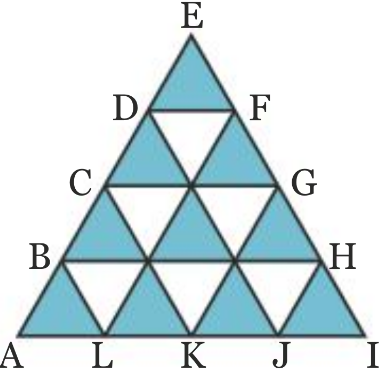
\includegraphics[scale=.3]{triangles.png}
    \end{center}
  \end{minipage}
\end{app}

\subsection{Caractéristiques d'un vecteur}
\begin{defi}{Caractéristiques d'un vecteur}
  \begin{minipage}{.5\textwidth}
  Le vecteur $\vect{AB}$ est défini par
  \begin{itemize}
    \item \textbf{sa direction} : celle de la droite $\left( AB \right)$;
    \item \textbf{son sens} : de $A$ vers $B$;
    \item \textbf{sa norme} : la longueur du segment $\left[ AB \right]$.
  \end{itemize}
  \end{minipage}
  \begin{minipage}{.5\textwidth}
  \begin{center}
    \begin{tikzpicture}
      \draw[loosely dashed] (0,0) -- (1.5, .5);
      \draw[red, thick, -latex] (1.5,0.5) -- (4.5, 1.5);
      \draw[loosely dashed] (4.5,1.5) -- (6, 2);
      \node at (1.5, 0.8) {$A$};
      \node at (4.5, 1.8) {$B$};
    \end{tikzpicture}
  \end{center}
  \end{minipage}
\end{defi}

\begin{app}
  \begin{minipage}[]{.5\textwidth}
    Sur la figure ci-contre, on a représenté les points $A, B, C, C', D, E, F$
    et $F'$, placés sur des droites parallèles.
    \begin{enumerate}
      \item Citer les vecteurs ayant le même sens.
      \item Citer les vecteurs ayant la même norme.
      \item Citer les vecteurs ayant la même direction.
      \item Donner l'image du point $F$ par la translation de vecteur
        $\vect{AB}$.
    \end{enumerate}
  \end{minipage}
  \begin{minipage}[]{.5\textwidth}
    \begin{center}
      \begin{tikzpicture}
        \draw[thick, dashed] (0,0) -- (1, 1/3);
        \draw[thick, green!50!black, -latex] (5, 5/3) -- (1,1/3);
        \draw[thick, dashed] (5, 5/3) -- (6,2);
        \node at (.8, .6) {$E$};
        \node at (5.1, 2) {$D$};

        \draw[thick, dashed] (0,1) -- (2, 5/3);
        \draw[thick, red, -latex] (2, 5/3) -- (4, 7/3);
        \draw[thick, dashed] (4, 7/3) -- (6,3);
        \node at (1.8, 1.9) {$C$};
        \node at (4, 2.6) {$C'$};

        \draw[thick, dashed] (0,2) -- (3, 3);
        \draw[thick, orange, -latex] (5, 11/3) -- (3, 3);
        \draw[thick, dashed] (6,4) -- (5, 11/3);
        \node at (3.2, 3.3) {$F$};
        \node at (5, 3.9) {$F'$};

        \draw[thick, dashed] (0,3) -- (1, 10/3);
        \draw[thick, red, -latex] (1, 10/3) -- (3,4);
        \draw[thick, dashed] (3,4) -- (4, 13/3);
        \node at (.8, 3.6) {$A$};
        \node at (3.1, 4.3) {$B$};
      \end{tikzpicture}
    \end{center}
  \end{minipage}
\end{app}

\begin{notation}
  La \textbf{norme} du vecteur $\vect{AB}$ se note $||\vect{AB}||$.
\end{notation}

\subsection{Égalité de vecteurs}
\begin{defi}{Égalité de vecteurs}
  Deux vecteurs sont dits \textbf{égaux} s'ils ont la même direction, le même
  sens, et la même longueur.
\end{defi}

\begin{prop}~\\[-5mm]
  \begin{minipage}[]{.68\textwidth}
  Le quadrilatère $ABCD$ est un \textbf{parallélogramme} si et seulement si
  \[
    \vect{AB} = \vect{CD}.
  \]
\end{minipage}\hspace{-6mm}
  \begin{minipage}[]{.32\textwidth}
    \begin{center}
      \begin{tikzpicture}
        \draw[dashed] (0,0) -- (4, 1);
        \draw[dashed] (1,1) -- (5, 2);
        \draw[red, thick, -latex] (0,0) -- (1, 1);
        \draw[red, thick, -latex] (4,1) -- (5, 2);

        \node at (-.2, 0) {$A$};
        \node at (.6, .9) {$B$};
        \node at (4.1, .8) {$C$};
        \node at (5.1, 1.8) {$D$};
      \end{tikzpicture}
    \end{center}
  \end{minipage}
\end{prop}

\begin{app}
  \begin{minipage}[]{.3\textwidth}
    On place ci-contre les points $A, B, C, D, E, F, G, H$ dans un repère.
    \begin{enumerate}
      \item Le quadrilatère $ABDC$ est-il un parallélogramme ?
      \item Le quadrilatère $EFGH$ est-il un parallélogramme ?
    \end{enumerate}
  \end{minipage}
  \begin{minipage}[]{.7\textwidth}
    \begin{center}
      \begin{tikzpicture}
        \foreach \x in {0, ..., 20}{
          \draw[opacity=.5] (.5*\x, -.1) -- (.5*\x, 5.1);
        }
        \foreach \y in {0, ..., 10}{
          \draw[opacity=.5] (-.1, .5*\y) -- (10.1, .5*\y);
        }

        \point{5}{2.5}{black};
        \node at (5.25, 2.75) {$A$};

        \point{3}{1.5}{black};
        \node at (3.25, 1.75) {$B$};

        \point{6}{4.5}{black};
        \node at (6.25, 4.75) {$C$};

        \point{4}{3.5}{black};
        \node at (4.25, 3.75) {$D$};

        \point{9}{0}{black};
        \node at (9.25, 0.25) {$E$};

        \point{.5}{1}{black};
        \node at (.75, 1.25) {$F$};

        \point{2}{4.5}{black};
        \node at (2.25, 4.75) {$G$};

        \point{10}{3.5}{black};
        \node at (10.25, 3.75) {$H$};
      \end{tikzpicture}
    \end{center}
  \end{minipage}
\end{app}

\begin{rmq}
  \textbf{Attention !} Le sens des lettres dans la propriété précédente ($ABDC$)
  n'est pas le sens habituel ($ABCD$).
\end{rmq}%~\\[-12mm]
\vspace{-.5cm}
\begin{rmq}
  Le parallélogramme peut éventuellement être aplati, c'est-à-dire que tous ses
  points soient alignés sur une même droite. La propriété reste vraie.
\end{rmq}
\vspace{-.5cm}

\subsection{Vecteurs opposés}
\begin{defi}{Vecteur opposé}
  Le \textbf{vecteur opposé} au vecteur $\vect u$, noté $-\vect u$, est le
  vecteur qui possède la même direction et la même norme que le vecteur $\vect
  u$, mais qui a un sens opposé.
\end{defi}
\begin{prop}~\\[-2mm]
  \begin{minipage}[]{.6\textwidth}
  L'opposé du vecteur $\vect{AB}$ est le vecteur $\vect{BA}$. On a donc
  \[
    -\vect{AB} = \vect{BA}.
  \]
  \end{minipage}
  \begin{minipage}[]{.4\textwidth}
    \begin{center}
      \begin{tikzpicture}
        \draw[red, -latex, thick] (0,0) -- (4, 1);
        \draw[blue, latex-, thick] (.025,-.1) -- (4.025, .9);
        \node at (-.2, 0) {$A$};
        \node at (4.2, 1.1) {$B$};
      \end{tikzpicture}
    \end{center}
  \end{minipage}
\end{prop}
    
\section{Propriétés des vecteurs}
\subsection{Milieu et vecteur}
\begin{prop}
  Pour tous points du plan $A$ et $B$, $\vect{AM}=\vect{MB}$ si et seulement si
  $M$ est le milieu de $[AB]$.
\end{prop}

\begin{app}
  Soient $A(2; 5)$, $M(6; 7)$ et $B(10; 9)$.
  \begin{enumerate}
    \item Calculer les vecteurs $\vect{AM}$ et $\vect{MB}$.
    \item Le point $M$ est-il le milieu de $\left[ AB \right]$ ?
    \item Calculer les coordonnées du point $C$ tel que $B$ soit le milieu de
      $\left[ AC \right]$.
  \end{enumerate}
\end{app}

\subsection{Représentant d'un vecteur}
\begin{defi}{Représentant}
  \begin{minipage}[]{.5\textwidth}
    Lorsque $\vect{AB}=\vect{CD}=\vect{EF}$, alors on dit que les vecteurs
    $\vect{AB}$, $\vect{CD}$ et $\vect{EF}$ sont des représentants d'un même
    vecteur que l'on peut également noter avec une seule lettre minuscule $\vect
    u$, $\vect v$, $\ldots$, indépendamment des deux points. On note alors
    \[
    \vect u=\vect{AB}=\vect{CD}=\vect{EF}.
  \]
  \end{minipage}
  \begin{minipage}[]{.5\textwidth}
    \begin{center}
      \begin{tikzpicture}
        \draw[red, thick, -latex] (0,0) -- (3, 1);
        \draw[blue, thick, -latex] (0,1) -- (3, 2);
        \draw[green!50!black, thick, -latex] (1,2) -- (4, 3);
        \draw[orange!50!black, thick, -latex] (-2, 2) -- node[above] {$\vect u$} (1, 3);

        \node[red] at (-.2, 0) {$A$};
        \node[red] at (3.2, 1) {$B$};

        \node[blue] at (-.2, 1) {$C$};
        \node[blue] at (3.2, 2) {$D$};

        \node[green!50!black] at (.8, 2) {$E$};
        \node[green!50!black] at (4.2, 3) {$F$};
      \end{tikzpicture}
    \end{center}
  \end{minipage}
\end{defi}
\begin{rmq}
  Un vecteur admet une \textbf{infinité} de représentants.
\end{rmq}~\\[-15mm]
\subsection{Sommes de vecteurs}
\begin{defi}{Somme de vecteurs}~\\[-4mm]
  \begin{minipage}[]{.5\textwidth}
    La \textbf{somme} de deux vecteurs $\vect u$ et $\vect v$ et le vecteur
    $\vect u+\vect v$ associé à la translation obtenue par la translation de
    vecteur $\vect u$ suivie de la transalation de vecteur $\vect v$.
  \end{minipage}
  \begin{minipage}[]{.5\textwidth}
    \begin{center}
      \begin{tikzpicture}
        \draw[green!50!black, -latex, thick] (0,0) -- (3, 2);
        \draw[green!50!black, -latex, thick] (-.5,.5) -- node[above left]
        {$\vect u$} (2.5, 2.5);
        
        \draw[blue, -latex, thick] (3,2) -- (5, 1);
        \draw[blue, -latex, thick] (3.5,2.5) -- node[above right] {$\vect v$}
        (5.5, 1.5);

        \draw[red, -latex, very thick] (0,0) -- node[above] {$\vect u+\vect
        v$} (5, 1);
      \end{tikzpicture}
    \end{center}
  \end{minipage}
\end{defi}

\begin{defi}{Différence de vecteurs}~\\[-6mm]
  \begin{minipage}[]{.5\textwidth}
  La \textbf{différence} de deux vecteurs $\vect u$ et $\vect v$ est le vecteur
  $\vect u-\vect v=\vect u+\left( -\vect v \right)$. Cela signifie que
  soustraire un vecteur revient à additionner son opposé.
  \end{minipage}
  \begin{minipage}[]{.5\textwidth}
    \begin{center}
      \begin{tikzpicture}
        \draw[green!50!black, -latex, thick] (0,0) -- (3, 2);
        \draw[green!50!black, -latex, thick] (-2.5,1.5) -- node[above left]
        {$\vect u$} (.5, 3.5);
        
        \draw[blue, -latex, thick] (3,2) -- (1, 3);
        \draw[blue, -latex, thick] (1.5,3.5) -- node[above right] {$\vect v$}
        (3.5, 2.5);

        \draw[red, -latex, very thick] (0,0) -- node[left] {$\vect u-\vect
        v$} (1, 3);
      \end{tikzpicture}
    \end{center}
  \end{minipage}
\end{defi}

\begin{propnom}{Relation de Chasles}~\\[-8mm]
  \begin{minipage}[]{.5\textwidth}
    Pour tous points $A$, $B$ et $C$ du plan, on a
  \[
    \vect{AB}+\vect{BC} = \vect{AC}.
  \]
  \end{minipage}
  \begin{minipage}[]{.5\textwidth}
  \begin{center}
    \begin{tikzpicture}[scale=1.08]
      \draw[blue, thick, -latex] (0,0) -- node[above left] {$\vect{BC}$} (-2, -1);
      \draw[red, thick, -latex] (2,-2) -- node[below] {$\vect{AC}$} (-2, -1);
      \draw[green!50!black, thick, -latex] (2,-2) -- node[above right]
      {$\vect{AB}$} (0, 0);

      \node at (0,0.2) {$B$};
      \node at (-2.3,-1) {$C$};
      \node at (2.2,-2) {$A$};
    \end{tikzpicture}
  \end{center}
  \end{minipage}
\end{propnom}

\begin{propnom}{Propriété du parallélogramme}
    Pour tous points $A$, $B$ et $C$ du plan, on a
  \[
    \vect{AB}+\vect{BC} = \vect{AD}
  \]
  si, et seulement si, $ABDC$ est un parallélogramme.
\end{propnom}

\begin{app}
  Soit $A, B, C, D$ des points du plan.
  \begin{enumerate}
    \item Simplifier le vecteur $\vect{BA}+\vect{AC}+\vect{CD}$.
    \item Simplifier le vecteur $\vect{AD}+\vect{BC}+\vect{AB}$.
  \end{enumerate}
\end{app}

\section{Vecteurs dans un repère}
\begin{defi}{Coordonnées d'un vecteur}
  Dans un repère $(0; I, J)$, les \textbf{coordonnées du vecteur} $\vect u$ sont
  les coordonnées de l'unique point $M$ tel que $\vect{OM}=\vect u$.
\end{defi}
\begin{prop}
  Dans si repère, si $A(x_A, y_A)$ et $B(x_B, y_B)$ alors $\vect{AB}$ a pour
  coordonnées $\vect{AB}\begin{pmatrix}x_B-x_A\\y_B-y_A\end{pmatrix}$. On écrit
  aussi $\vect{AB}(x_B-x_A,y_B-y_A)$.
\end{prop}
\begin{app}
  Soit $A(1;2)$, $B(2, -2)$ et $C(-3, 0)$ trois points d'un repère du plan $(O;
  I, J)$.
  \begin{enumerate}
    \item Faire une figure et y placer les points $A, B, C$.
    \item Donner les coordonnées de $\vect{AB}$ ainsi que le représentant
      d'origine $O$ de ce vecteur.
    \item Donner les coordonnées de $\vect{AC}$ ainsi que le représentant
      d'origine $O$ de ce vecteur.
  \end{enumerate}
\end{app}

\begin{prop}
  Deux vecteurs sont égaux si, et seulement si, ils ont les mêmes coordonnées.
\end{prop}

\begin{app}
  Soient $A(-3; 1)$, $B(2; 2)$, $C(4; 5)$ et $D(9; 6)$. Le quadrilatère $ABDC$
  est-il un parallélogramme ?
\end{app}

\subsection{Coordonnées d'une somme}
\begin{prop}
  Soient $\vect r\begin{pmatrix}x\\y\end{pmatrix}$ et
  $\vect s\begin{pmatrix}x'\\y'\end{pmatrix}$ deux vecteurs d'un repère du plan.
  Les coordonnées de $\vect r+\vect s$ sont alors
  $\begin{pmatrix}x+x'\\y+y'\end{pmatrix}$.
\end{prop}

\begin{app}
  Soient $A(1; 1)$, $B(-2; 3)$, $C(4; -1)$.
  \begin{enumerate}
    \item Calculer les coordonnées de $\vect{AB}$, $\vect{BC}$ et
      $\vect{AC}$.
    \item Calculer $\vect{AB}+\vect{BC}$ gr\^ace aux coordonnées.
    \item Quelle égalité retrouve-t-on ?
  \end{enumerate}
\end{app}

\subsection{Produit d'un vecteur par un réel}
\begin{defi}{Produit d'un vecteur par un réel}
  Soit $\lambda\in\mathbb{R}$ un réel et $\vect u$ un vecteur de coordonnées
  $\begin{pmatrix}x\\y\end{pmatrix}$. Le vecteur $\lambda\vect u$ a pour
  coordonnées $\begin{pmatrix}\lambda x \\ \lambda y \end{pmatrix}$.
\end{defi}
\begin{prop}
  Soient $\lambda, \lambda'\in\mathbb{R}$ deux nombres réels, $\vect u$ et $\vect w$ deux vecteurs. On a
  \begin{align*}
    \textbf{1.}\;& \lambda\left( \vect u +\vect w \right) = \lambda\vect
    u+\lambda\vect w &
    \textbf{2.}\;& \left( \lambda+\lambda' \right)\vect u = \lambda\vect
    u+\lambda'\vect u &
    \textbf{3.}\;& \lambda\left( \lambda'\vect u\right) = \left( \lambda\lambda'
    \right)\vect u
  \end{align*}
\end{prop}

\begin{app}
  Soit deux vecteurs $\vect u $ et $\vect v$ données par $\vect u\begin{pmatrix}
    2\\-1\end{pmatrix}$ et $\vect v\begin{pmatrix}5\\3\end{pmatrix}$.
  \begin{enumerate}
    \item Calculer $2\vect u$ et $3\vect v$.
    \item Calculer le vecteur $\vect w$ donné par $\vect w=\vect v-3\vect u$.
    \item Soit $A(-7; 1)$. Déterminer les coordonnées du point $M$ tel que $AM =
      \vect u-\vect v$.
  \end{enumerate}
\end{app}

\end{document}
